\section{求解误差与计算成本}
\label{sec:smooth-accuracy-cost}

上一节比较的是单步。一个算法要迭代许多轮，两个算法之间的比较还要回答更多问题。这就需要回答：两种方法求解同一个问题，怎样比较才算数？第~\ref{chap:optimization}章规定了怎样衡量一个近似解，本节把它接到迭代过程上，再加上计算量的统计。

\paragraph{结论会随口径翻转}
在例~\eqref{eq:smooth-running}上，从$\bm{x}^{(0)}=(9,1)$出发，用五种步长规则运行负梯度方法，直到目标差不超过$10^{-6}$。表~\ref{tab:smooth-cost-run}列出外层轮数和各种读取次数。这里算总次数时把一次函数值、一次梯度、一次矩阵向量积各记为一个单位，因为对二次目标它们都要做一次矩阵向量积。

\begin{BookInlineTable}
  \centering
  \begin{tabular}{@{}lrrrrr@{}}
    \toprule
    步长规则 & 轮数$T$ & 函数值 & 梯度 & 矩阵向量积 & 总次数\\
    \midrule
    固定$\alpha=1/L$ & 75 & 0 & 76 & 0 & 76\\
    固定$\alpha=0.2$ & 40 & 0 & 41 & 0 & 41\\
    精确线搜索 & 40 & 0 & 41 & 40 & 81\\
    回溯，$\alpha_0=1$ & 23 & 71 & 24 & 0 & 95\\
    回溯，初值放大 & 31 & 65 & 32 & 0 & 97\\
    \bottomrule
  \end{tabular}
  \caption{例~\eqref{eq:smooth-running}上负梯度方法达到目标差不超过$10^{-6}$的计算量。固定步长$0.2=2/(L+\mu)$要同时知道$L$和$\mu$；梯度数包含初始点。回溯的函数值数包含初始点和所有被拒绝的试探。}
  \label{tab:smooth-cost-run}
\end{BookInlineTable}

按轮数看，回溯最少，比第二名少了将近一半。按总次数看，排序几乎反过来：回溯不如不做任何试探的固定步长，而精确线搜索也花掉了比固定步长$0.2$多一倍的计算。图~\ref{fig:smooth-cost-convergence}中两张图的曲线次序不同，差别只在横轴。

\begin{BookInlineFigure}
  \centering
  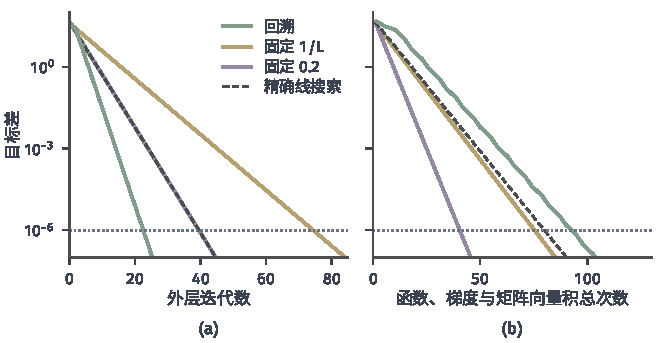
\includegraphics[width=112mm]{figures/05-optimization/02-smooth-optimization/matplotlib/smooth-cost-convergence/figure.pdf}
  \caption{同一组运行的两种横轴，目标见例~\eqref{eq:smooth-running}，纵轴是目标差，点线是$10^{-6}$。(a)横轴是外层迭代数，绿色的回溯最快。(b)横轴是函数值、梯度与矩阵向量积的总次数，紫色的固定步长$0.2$最快。回溯曲线在(b)中被试探次数拉长。}
  \label{fig:smooth-cost-convergence}
\end{BookInlineFigure}

这个例子不说明哪种规则更好。若函数值远比梯度便宜，或者$L$和$\mu$未知，结论都要改变。它说明的是：不交代口径的比较没有意义。比较之前要固定三件事：用什么量衡量误差，算法交出哪个点，计算量怎样累计。

\paragraph{误差标准}
第~\ref{chap:optimization}章的三种指标在这里要按问题类型选择。凸目标上驻点就是全局最优解，目标差$e_f=f(\bm{x})-f^\star$有明确的含义，比较时通常用它，保证也通常写成目标差的形式。

一般非凸目标的$f^\star$既算不出来，算法也无法保证接近它。这时能够断言的只有驻点残差$e_g=\lVert\nabla f(\bm{x})\rVert_2$：它只回答一阶条件差多少，不说明是局部还是全局的最小点，这在第~\ref{chap:saddle-points}章还要细分。

两种标准之间的换算，依据是第~\ref{chap:optimization}章三种误差的换算和本章的式~\eqref{eq:smooth-gap-gradient}。由目标差推梯度只要$L$：
\[
 e_g\leq\sqrt{2L\,e_f}.
\]
由梯度推目标差还要曲率下界$\mu$：
\[
 e_f\leq\frac{e_g^2}{2\mu}.
\]

例~\eqref{eq:smooth-running}中$L=9$，$\mu=1$。目标差$10^{-6}$只保证梯度不超过$\sqrt{18}\times10^{-3}\approx4.2\times10^{-3}$；梯度$10^{-3}$保证目标差不超过$5\times10^{-7}$。所以两种标准的“同样精度”并不相同，比较时不能混用。

\paragraph{一步下降怎样累积成驻点保证}
前面三种步长规则的下降保证都能写成同一个形式：一步的下降量不少于$c\lVert\bm{g}^{(t)}\rVert_2^2$，$c$是正常数。把这种形式累加起来，就得到不依赖凸性的驻点保证。

\begin{lemma}[累加下降]
\label{lem:smooth-telescoping}
设$f$下有界，$f_{\inf}=\inf f$，常数$c>0$，迭代满足
\begin{equation}
 f(\bm{x}^{(t)})-f(\bm{x}^{(t+1)})\geq c\lVert\bm{g}^{(t)}\rVert_2^2,\qquad t=0,\ldots,T-1.
 \label{eq:smooth-uniform-decrease}
\end{equation}
则
\begin{equation}
 \min_{0\leq t<T}\lVert\bm{g}^{(t)}\rVert_2^2\leq\frac{f(\bm{x}^{(0)})-f_{\inf}}{cT}.
 \label{eq:smooth-telescoping}
\end{equation}
\end{lemma}

\begin{proof}
对$t=0,\ldots,T-1$累加式~\eqref{eq:smooth-uniform-decrease}，左端相消，得到
\[
 f(\bm{x}^{(0)})-f(\bm{x}^{(T)})\geq c\sum_{t=0}^{T-1}\lVert\bm{g}^{(t)}\rVert_2^2\geq cT\min_{0\leq t<T}\lVert\bm{g}^{(t)}\rVert_2^2.
\]
左端不超过$f(\bm{x}^{(0)})-f_{\inf}$，移项即得。
\end{proof}

由式~\eqref{eq:smooth-telescoping}，要使$\min_t\lVert\bm{g}^{(t)}\rVert_2\leq\varepsilon$，轮数只要达到
\begin{equation}
 T\geq\frac{f(\bm{x}^{(0)})-f_{\inf}}{c\,\varepsilon^2}.
 \label{eq:smooth-iteration-bound}
\end{equation}

下一章将用这种累加结果处理一般非凸情形。三种规则对应的常数$c$如下，方向都取负梯度，Wolfe的情形允许夹角满足$\cos\theta^{(t)}\geq\delta>0$的一般方向，此时下降量与$\lVert\bm{g}^{(t)}\rVert_2^2$的比例同样有正下界：
\[
 \begin{aligned}
 \text{固定步长}\ \alpha=\tfrac{1}{L}:&\quad c=\frac{1}{2L},\\
 \text{回溯}:&\quad c=\min\Bigl\{c_1\alpha_0,\ \frac{2\rho c_1(1-c_1)}{L}\Bigr\},\\
 \text{Wolfe}:&\quad c=\frac{c_1(1-c_2)\delta^2}{L}.
 \end{aligned}
\]

代入例~\eqref{eq:smooth-running}的数值，看看这种保证和实际运行的距离。$f(\bm{x}^{(0)})-f_{\inf}=45$，$L=9$，取$\varepsilon=10^{-3}$。固定步长$1/L$的$c=1/18$，式~\eqref{eq:smooth-iteration-bound}要求$T\geq8.1\times10^8$，而实际只用了$78$轮。

差距这样大是因为式~\eqref{eq:smooth-telescoping}对任意$L$光滑的目标成立，包括最坏的非凸函数，它没有用到这个例子的二次结构。因此要区分两种“轮数”：理论界是对一类问题的最坏保证，实测值是在一个问题上的表现。两者都有用，但不能相互替代。

\paragraph{返回哪个迭代点}
式~\eqref{eq:smooth-telescoping}左端是历史上最小的梯度，所以保证的是某一轮的点，不一定是最后一轮。这个区别不是形式上的。取$f(x)=1-\cos x$，固定步长$\alpha=1/L=1$，从$x^{(0)}=3$出发。前四轮的迭代值如下：
\[
 \begin{aligned}
 x&:\ 3,\ 2.859,\ 2.580,\ 2.047,\ 1.159,\\
 f&:\ 1.990,\ 1.960,\ 1.846,\ 1.459,\ 0.600,\\
 \lvert f'\rvert&:\ 0.141,\ 0.279,\ 0.533,\ 0.889,\ 0.916.
 \end{aligned}
\]

目标在下降，梯度却在上升，如图~\ref{fig:smooth-best-vs-last}。起点靠近山顶$x=\pi$，那里梯度很小；离开山顶的过程中坡度越来越陡。由此可见，下降引理只控制目标的单调性，不控制梯度的单调性。

\begin{BookInlineFigure}
  \centering
  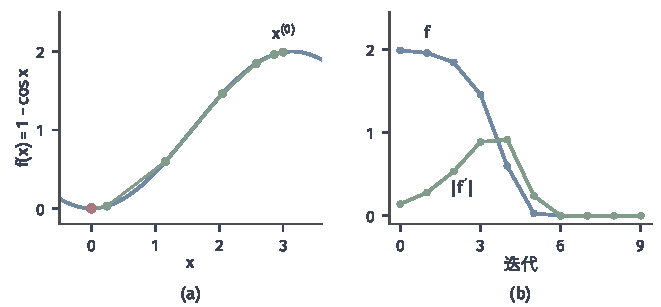
\includegraphics[width=112mm]{figures/05-optimization/02-smooth-optimization/matplotlib/smooth-best-vs-last/figure.pdf}
  \caption{目标单调下降时梯度可以先升后降。$f(x)=1-\cos x$，$\alpha=1$，$x^{(0)}=3$。(a)曲线上的迭代点（绿色）。(b)目标值（蓝）单调下降，导数绝对值（绿）在前四轮上升，到第$5$轮后才迅速下降。}
  \label{fig:smooth-best-vs-last}
\end{BookInlineFigure}

这个例子还有另一面：若容差取$\varepsilon=0.2$，初始点$x^{(0)}=3$本身就能通过检验，而它靠近的是极大点。所以驻点残差小只是一阶条件的说明，它不区分山顶与谷底。

报告结果时，常见的返回规则有三种。一是最后一轮$\bm{x}^{(T)}$，凸目标上的多数保证针对它，不需要记录历史。二是历史最佳，即目标值或梯度范数最小的那一轮，式~\eqref{eq:smooth-telescoping}对应这种规则，需要额外记录。三是停止点，第一次满足$\lVert\bm{g}^{(t)}\rVert_2\leq\varepsilon$的那一轮，停止时它就是历史上第一个合格的点。

下一章有些方法的目标值不单调，最后一轮不一定是最好的一轮，这时必须说明按哪条规则返回。

\paragraph{停止精度}
实际运行时$f^\star$未知，停止规则只能用可计算的量。梯度范数是首选，第~\ref{chap:optimization}章的相对标准，即把容差乘以$\max\{1,\lVert\bm{g}^{(0)}\rVert_2\}$，能够避免目标整体缩放带来的问题。步长或目标变化量太小的检验只能作辅助：回溯在一轮中接受了很小的步长时，位移也很小，但这只反映这一轮的步长，并不说明点已接近驻点。

容差还要与计算机的能力相称。在双精度浮点数中，$1+\delta$对$\delta$小于约$1.1\times10^{-16}$的数等于$1$。考虑$f(x)=1+\frac12x^2$，$x=10^{-9}$时，真实值$1+5\times10^{-19}$与$1$无法区分。

因此在最优值附近，比较函数值只能把点确定到约$\sqrt{\text{机器精度}}\approx10^{-8}$的范围，Armijo检验也就失去了分辨力。梯度$f'(x)=x$却还能算准。这说明可达到的精度取决于用什么量作判断，容差设得比判断量的计算误差还小是没有意义的。

\paragraph{总计算量}
选定误差标准和返回规则后，记$T(\varepsilon)$为达到精度$\varepsilon$所需的外层轮数。总计算量要把每一轮实际做过的所有运算加起来。设一次函数值、梯度、矩阵向量积的代价分别是$c_f,c_g,c_{\mathrm{mv}}$，第$t$轮有$n^{(t)}$次函数计算、$k^{(t)}$次内层矩阵向量积、线性代数运算量$c_{\mathrm{la}}^{(t)}$，于是
\begin{equation}
 W(\varepsilon)=\sum_{t=0}^{T(\varepsilon)-1}\Bigl(n^{(t)}c_f+c_g+k^{(t)}c_{\mathrm{mv}}+c_{\mathrm{la}}^{(t)}\Bigr).
 \label{eq:smooth-total-work}
\end{equation}

式中$n^{(t)}$包含被拒绝的试探；$k^{(t)}$是用迭代法解内层线性方程时的步数。图~\ref{fig:smooth-work-accounting}显示了每一轮的三部分怎样累加成$W(\varepsilon)$。

\begin{BookInlineFigure}
  \centering
  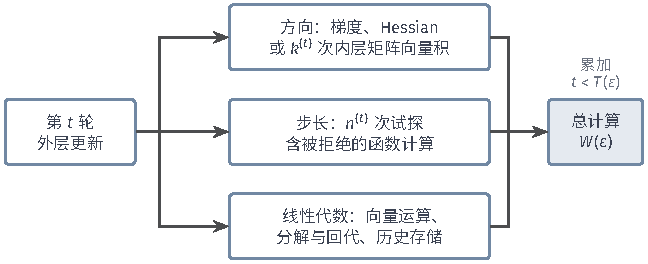
\includegraphics[width=108mm]{figures/05-optimization/02-smooth-optimization/tikz/smooth-work-accounting/figure.pdf}
  \caption{总计算量的组成。每一轮外层更新包含方向计算、步长试探和线性代数三部分，对达到精度所需的全部轮次累加，得到$W(\varepsilon)$。迭代轮数只决定累加的项数，每项的大小要另外统计。}
  \label{fig:smooth-work-accounting}
\end{BookInlineFigure}

\paragraph{单次更新的代价}
不同方法的每轮代价差别很大。表~\ref{tab:smooth-per-iter}按$n$维稠密问题列出下一章起要用到的几类操作。其中第三行的方向要解线性方程$\bm{H}\bm{d}=-\bm{g}$：可以分解矩阵直接解，也可以用迭代法只做矩阵向量积、解到一定精度为止，后者就是内层求解。

\begin{BookInlineTable}
  \centering
  \begin{tabular}{@{}lll@{}}
    \toprule
    一轮更新的操作 & 运算量 & 存储\\
    \midrule
    梯度与向量更新 & $c_g+O(n)$ & $O(n)$\\
    回溯线搜索 & 再加$n^{(t)}c_f$ & $O(n)$\\
    分解Hessian解方程 & $c_H+\frac13n^3+O(n^2)$ & $O(n^2)$\\
    内层迭代解方程 & $k^{(t)}c_{\mathrm{mv}}+O(k^{(t)}n)$ & $O(n)$\\
    \bottomrule
  \end{tabular}
  \caption{一轮更新中常见操作的代价，$c_H$是形成一次Hessian的代价，分解按Cholesky计。单轮代价低的方法不一定总代价低。}
  \label{tab:smooth-per-iter}
\end{BookInlineTable}

单轮代价和总代价是两个不同的量。用线性方程的三种解法作对照最清楚，$\bm{H}\bm{x}=\bm{b}$等价于最小化$\frac12\bm{x}^\top\bm{H}\bm{x}-\bm{b}^\top\bm{x}$，设$\bm{H}$稠密、$\kappa=L/\mu$，要把目标差缩小到初值的$\varepsilon$倍。下面三个数都是最坏情形的估计。

梯度下降取$\alpha=1/L$时，每个特征方向的乘数绝对值不超过$1-1/\kappa$，目标差每轮至少乘$(1-1/\kappa)^2$，所以轮数约是
\[
 T_{\mathrm{GD}}\approx\frac{\kappa}{2}\ln\frac{1}{\varepsilon}.
\]

共轭梯度法的能量范数误差不超过$2q^T\lVert\bm{e}^{(0)}\rVert_{\bm{H}}$，其中$q=(\sqrt\kappa-1)/(\sqrt\kappa+1)$，这一结论的证明可参考\BookChapterRef{chap:krylov-methods}{卷二第15章“Krylov子空间法”}。由$\ln(1/q)\approx2/\sqrt\kappa$，轮数约是
\[
 T_{\mathrm{CG}}\approx\frac{\sqrt\kappa}{4}\ln\frac{4}{\varepsilon}.
\]

两者每轮都是一次矩阵向量积，约$2n^2$次运算。Cholesky分解约$n^3/3$次运算，外加回代$2n^2$次。取$\kappa=100$，$\varepsilon=10^{-6}$，代入得到
\[
 T_{\mathrm{GD}}\approx691,\qquad T_{\mathrm{CG}}\approx39.
\]

单轮代价是$n^3/3$与$2n^2$之比，单看一轮，迭代法便宜得多。把轮数算上，令$2n^2T=n^3/3$，交叉点在$n=6T$：
\[
 n_{\mathrm{GD}}\approx4146,\qquad n_{\mathrm{CG}}\approx234.
\]

图~\ref{fig:smooth-work-crossover}画出这三条总运算量曲线。维数低于交叉点时，一次分解比许多轮便宜的迭代总和更省。稀疏矩阵的矩阵向量积只需与非零元数成比例的运算，分解却可能产生填充，这时交叉点又会移动，比较要重新做。

\begin{BookInlineFigure}
  \centering
  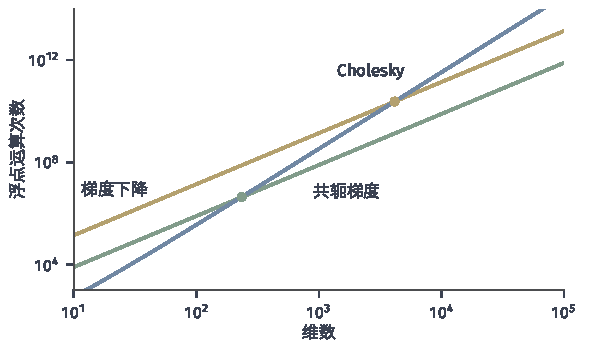
\includegraphics[width=100mm]{figures/05-optimization/02-smooth-optimization/matplotlib/smooth-work-crossover/figure.pdf}
  \caption{稠密对称正定方程的总运算量估计，$\kappa=100$，$\varepsilon=10^{-6}$。黄线为梯度下降（$691$轮），绿线为共轭梯度（$39$轮），每轮$2n^2$次运算；蓝线为Cholesky分解加回代。两个点是迭代法与分解的交叉位置，$n\approx4146$和$n\approx234$。}
  \label{fig:smooth-work-crossover}
\end{BookInlineFigure}

\paragraph{内层求解}
外层方法里嵌套内层迭代时，式~\eqref{eq:smooth-total-work}的$k^{(t)}$不能忽略。作为教学算例，假设一种用Hessian的方法外层只要$6$轮，每轮用$20$次矩阵向量积近似解方程，矩阵向量积与梯度代价相同；另一种只用梯度的方法要$60$轮。按外层轮数比较前者少$10$倍，按读取次数比较则是
\[
 6\times(1+20)=126,\qquad 60\times1=60.
\]
结论反了过来。内层容差也属于口径的一部分：内层解得越精确，外层轮数可能越少，每轮却越贵，第~\ref{chap:second-order-methods}章会讨论两者的权衡。

\paragraph{比较时要报告的内容}
把上面的要求列在一起，就是本卷后面比较算法时使用的口径，见表~\ref{tab:smooth-report}。按表中各项报告，读者才能判断两组数字是否可比。

\begin{BookInlineTable}
  \centering
  \begin{tabular}{@{}ll@{}}
    \toprule
    项目 & 需要交代的内容\\
    \midrule
    问题与起点 & 目标的结构、维数、初始点\\
    误差标准 & 目标差或驻点残差，绝对或相对容差\\
    返回规则 & 最后一轮、历史最佳或停止点\\
    外层统计 & 达到容差的轮数$T(\varepsilon)$\\
    读取统计 & 函数值、梯度、Hessian、矩阵向量积的次数\\
    被拒绝的试探 & 计入函数计算次数\\
    线性代数 & 分解、回代、内层迭代的运算量和存储\\
    结论类型 & 最坏情形的理论界，或特定问题上的实测值\\
    \bottomrule
  \end{tabular}
  \caption{比较优化算法时的报告项目。同一项目口径不同的两组结果不能直接比较。}
  \label{tab:smooth-report}
\end{BookInlineTable}
